\subsection{Locality-Sensitive Hash Functions} \label{subsec:locality-sensitive-hashes}

Introduced by Indyck and Motwani in 1998 \cite{indyk_approximate_1998} as an algorithm that solves the approximate nearest neighbour problem (ANN), locality-sensitive hashing (LSH) has since been extensively researched and is now considered among the state of the art for approximate searches in high-dimensional spaces.\footnote{See \cite{nagarkar2021exploring} for an exhaustive survey of NN-Search Techniques.} The basic idea of the approach is to partition the input data using a hash function that is sensitive to the location of the input within the metric space. This way, similar inputs collide with a higher probability than inputs that are far apart. Thus, LSH exhibits fundamental differences to conventional hash functions \footnote{In the following, cryptographic and non-cryptograhpic hash functions are referred to as conventional hashing.}, although the most general definition applies to both.

A hash function is a function that maps a large input set to a smaller target set. The elements of the input set are called \textit{messages} or \textit{keys} and may be of arbitrary different lengths. The elements of the target set are called \textit{digests} or \textit{hash values} and are of fixed size length. More specifically, we define a hash function as $h: A \rightarrow B : \bm{p} \mapsto \bm{u}$ where $A \subset \mathbb{R}^d$ with $d \in \mathbb{N}$ is the input set and $B=\{0, 1\}^k$ with $k \in \mathbb{N}$ the target set of all bit sequences of fixed size $k$, with $k < d$. Furthermore, a hash table is defined by a hash function $h$, that maps the keyspace $K$ into the slots of a hash table $T[0 \,.\,.\, S-1], S \in \mathbb{N}$, i.e. $h: K \rightarrow \{0, 1, \dots, S-1\}$ with $S \ll |K|$. Thus, a message with key $k \in K$ hashes to slot $h(k)$. Additionally, $h(k)$ is the hash value of the key $k$ \cite[256]{cormen2022introduction}.


% 1. Give formal definitions of Hash function and Hash table
% 2. Explain the difference of conventional hash function and LSH
% 3. Explain the big picture of the algorithm
%%%%%%%%%%%%%%%%%%%%%%%%%%%%%%%%%%%%%%


Typically,conventional hashing is used for the realization of, e.g. hash tables, data integrity checks, error correction methods or database indexes. Depending on the application, different requirements are imposed on the utilized hash function. In this context, the most important property of a hash function is the probability of a \textit{collision}. A collision occurs when two keys $\bm{p}_1 \neq \bm{p}_2$ are projected onto the same hash value $\bm{u} = h(\bm{p}_1) = h(\bm{p}_2)$.

For example, cryptographic hash functions are used in systems, where adversaries try to break these systems. Thus, different security requirements are defined \cite[349]{williamcryptography}. In particular, these hash functions are designed to be resistant against collisions, which is the key difference to LSH. Applications that do not require the hash function to be resistant against adversaries, e.g. hash tables, caches or de-duplication, are usually implemented by using a hash function that exhibits relaxed guarantees on the security properties in exchange for significant performance improvements. Nevertheless, such non-cryptographic hash functions share the same idea with cryptographic hash functions.

Figure \ref{fig:hashing_differences} illustrates this difference. LSH projects similar inputs onto the same or near elements. In contrast, conventional hashing tries to distribute projections onto the elements of the target as randomly as possible.

\begin{figure}[t!]
    \centering
    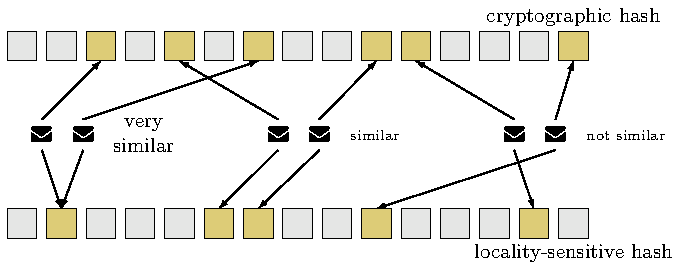
\includegraphics[width=0.8\linewidth]{tikz/hashing_differences.pdf}
    \caption{Cryptographic hash function and locality-sensitive hash function exhibit different properties for the probability of collisions.}
    \label{fig:hashing_differences}
\end{figure}




%%%%%%%%%%%%%%%%%%%%%%%%%%%%%%%%%%%%%%


% explain the idea of LSH (reduce the search space and then pick a random p or do a linear scan within the reduced search space)

As a locality-sensitive hashing function can be constructed as a general concept, specific families of functions can be derived. We refer to a \textit{family} of hash functions $\mathcal{H}: A \rightarrow B$ as a collection of hash functions that have the same domain and range, share a basic structure and are only differentiated by constants. Three basic requirements are demanded for such a family of functions \cite[99]{leskovec_rajaraman_ullman_2014}.

\begin{enumerate}
    \item close pairs are to be hashed in to the same bucket with higher probability than distant pairs
    \item the functions need to be statistically independent, such that the product rule can be applied on the results of two or more functions; It is said, that these functions are combinable, such that functions can be build/combined/constructed that provide less fals positives and false negatives than single functions
    \item they need to be efficient, i.e. able to identify similar pairs in much less time than the time it takes to make a linear scan through all pairs (faster than exhaustive search)

\end{enumerate}

The first step is to define LSH generally. Applied on the $cR$-ANN, the first requirement states more specifically with high probability, two points $p$ and $q$ should hash to the same hash value if their distance at most $R$, i.e. $d(p,q) \leq R$. And if their distance is at least $cR$, the points should hash to different hash values, i.e. $d(p,q) > cR$. Thus,  A formal definition of a locality-sensitive hash function is given as follows \cite{andoni2006near}.

\begin{definition}[Locality-Sesitive Hash Function]
    Given a threshold $R \in \mathbb{R}^{>0}$, an approximation factor $c \in \mathbb{R}^{>1}$ and probabilities $P_1, P_2 \in \mathbb{R}^{\geq 0}$, a family $\mathcal{H} = \{h: A \rightarrow B$\} is called $(R, cR, P_1, P_2)$-sensitive if for any two points $p,q \in A$ and any hash function $h$ chosen uniformly at random from $\mathcal{H}$ the following conditions are satisfied:
        \[
        \setlength\arraycolsep{0pt}
        \renewcommand\arraystretch{1.2}
            \begin{array}{LCL}
                d(p,q) \leq R & \implies & P[h(p)=h(q)] \geq P_1, \\
                d(p,q) \geq cR & \implies & P[h(p)=h(q)] \leq P_2.
            \end{array}
        \]
\end{definition}

% Figure \ref{fig:lsh_probability}, depicts the expected behaviour of a locality sensitive function. 
Ideally, the gap between $P_1$ and $P_2$ should be as big as possible as depicted in Figure \ref{subfig:exact_probability}, which in fact represents an exact search, which is, as already discussed, no option due to its time and space requirements. Considering a single locality-sensitive function as shown in Figure \ref{subfig:lsh_probability}, where the probability gap between $P_1$ and $P_2$ is relatively close, the false negative rate would be relatively high. Increasing the gap would require to increase $c$ and lead to a high number of false positives. Therefore, a single function would provide only a tradeoff. But it is possible to increase $P_1$ close to $1$ and decrease $P_2$ close to $1/n$ while keeping $R$ and $cR$ fixed as shown in Figure \ref{subfig:lsh_probability_boosted} by introducing a process called \textit{amplification}.

\begin{figure}
    \centering
    \begin{subfigure}[b]{0.3\textwidth}
        \centering
        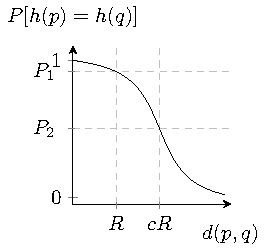
\includegraphics[width=\textwidth]{tikz/lsh_probability.pdf}
        \caption{Single LSH Function.}
        \label{subfig:lsh_probability}
    \end{subfigure}
    \hfill
    \begin{subfigure}[b]{0.3\textwidth}
        \centering
        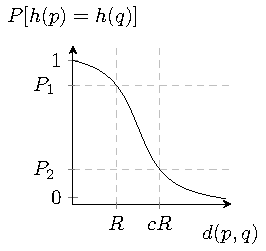
\includegraphics[width=\textwidth]{tikz/lsh_probability_boosted.pdf}
        \caption{Amplified LSH Function.}
        \label{subfig:lsh_probability_boosted}
        \end{subfigure}
        \hfill
        \begin{subfigure}[b]{0.3\textwidth}
            \centering
            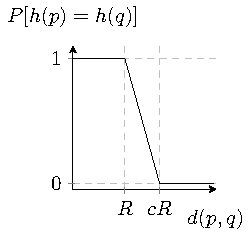
\includegraphics[width=\textwidth]{tikz/exact_probability.pdf}
            \caption{Exact Search}
            \label{subfig:exact_probability}
    \end{subfigure}
    \caption{The behaviour of a $(R, cR, P_1, P_2)$-sensitive function in (\ref{sub@subfig:lsh_probability}) and (\ref{sub@subfig:lsh_probability_boosted}) (adapted from \cite[100]{leskovec_rajaraman_ullman_2014}) approaching the ideal probability gap in (\ref{sub@subfig:exact_probability}) resembling the behaviour of an exact search.}
    \label{fig:lsh_probability}
\end{figure}

First reduce $P_2$ by applying logical AND (AND-construction on $\mathcal{H}$): sample $k$ hash functions indepedently from $\mathcal{H}$ and hash each point $p \in P$ to a $k$-dimensional vector with a new constructed function $g \in \mathcal{H}^k$:

\begin{equation}
    g(p) = [h_1(p), h_2(p), \dots, h_k(p)]
\end{equation}


Then by the independence of $h_1, \dots, h_k$ the product rule applies and for any two points $p$ and $q$, a collision occurs if and only if $h_i(p)=h_i(q)$ for all $i = \{1, \dots, k\}$. The probabilities are as follows:

\begin{align}
    P[h_i(p)=h_i(q)] \geq P_1 \implies P[g(p)=g(q)] \geq P_1^k \\
    P[h_i(p)=h_i(q)] \leq P_2 \implies P[g(p)=g(q)] \leq P_2^k 
\end{align}

By increasing $k$, $P_2$ can be arbitrarily decreased approaching $0$. However, such an AND-construction lowers both $P_1$ and $P_2$.There is another construction in order to improve $P_1$, the OR-construction: Using multiple families; specifically define $l \in \mathbb{N}$ functions $g_1, \dots, g_l$.

What is the probability that a collision occurs when hashing a point $p \in P$ witch each $g_j(p)$ for $j \in \{1, \dots, l\}$? Considering, that the algorithm is successful, when $p,q$ collide at least once for some $g_j$, the probability is

\begin{align}
    P[\exists j, g_j(p)=g_j(q)] &= 1 - P[\forall i, g_j(p) \neq g_j(q)] \\
                                &= 1 - P[g_j(p) \neq g_k(q)]^l \\
                                &\geq 1 - (1-P_1^k)^l
\end{align}

As the AND-construction lowered both $P_1$ and $P_2$, similarly the OR-construction rises both probablities. By choosing $k$ and $l$ judiciously, $P_2$ can be approached close to $0$ while $P_1$ approaches $1$. Both constructions may be concatenated in any order to manipulate $P_1$ and $P_2$. Of course, the more construction are used and the higher the values for the parameters $k$ and $l$ are picket, the larger the final function will be and it also takes longer to apply such a function. 


The algorithm is as follows. The construction of the data-structure:
\begin{itemize}
    \item construct $g_1, \dots, g_l$, each of length $k$
    \item hash each point $p \in P$ with each $g_j$ and store them in $l$ hash tables accordingly
\end{itemize}

Answering a query $q$:
\begin{itemize}
    \item compute $g_1(q), \dots, g_l(q)$. For each $g_j(q)$ identify those $p$, such that $g_j(p) = g_j(q)$. For each identified $p$ check if it answers $cR$-ANN with yes, i.e. $d(p, q) \leq cR$.
\end{itemize}

Naive betrachtungsweise des algorithmus:
Space complexity is $O(lnk)$, since there are $l$ hash tables, each with $n$ points, and for each point storing a $k-dim$ vector.

Lower bounds have been proven in \cite{motwani2006lower}

\begin{theorem}
    Let $(X,d)$ be a metric on a subset of $\mathbb{R}^d$. Given a $(R, cR, P_1, P_2)$-locality sensitive hash family $\mathcal{H}$ and write $\rho = \frac{\text{log}(1/P_1)}{\text{log}(1/P_2)}$. Then for $n = |X|$ and for any $n \geq \frac{1}{P_2}$ there exists a solution to the $cR$-ANN with space complexity $O(dn+n^{1+\rho})$ and query time of $O(n^{\rho})$
\end{theorem}


% Choose $k$ such that $P_2^k = \frac{1}{n}$. Then, the probability that a point $p$ that is far away from the query point $q$, i.e. $d(p,q) > cR$, maps to the same bucket as $q$ is relatively small.


% We use many independent hash functions from a family H to boost P_1 close to 1 and shrink P_2 close to 1/n


% In order for a $\mathcal{H}$ to be applicable for the $cR$-near neighbour problem, it has to satisfy the inequality $P_1 > P_2$.

